\chapter{Przegląd podobnych rozwiązań} 
Aplikacje do planowania podróży to często spotykane rozwiązanie ułatwiające organizowanie wyjazdów. Oferowane są dla systemów operacyjnych Android oraz iOS odpowiednio w serwisach Google Play i Apple Store. Przetestowano 4 przykładowe aplikacje, których podstawowe dane zawarte zostały w tabeli~\ref{tab:porównianie}.


\begin{table}[ht]
\captionof{table}{Dane testowanych aplikacji z dnia 15.03.2019\label{tab:porównianie}}
\centering
\begin{tabular}{ |c|c|c|c| }
\hline
\multirow{2}{6em}{\thead{\makecell{Nazwa \\ aplikacji}}} & \multicolumn{2}{c|}{\thead{Google Play}} & \thead{Apple Store}\\
\cline{2-4}
 & Średnia ocena & Ilość pobrań & Średnia ocena \\
\hline
TripIt: Travel Planner & \makecell{4.4/5 \\ (53217 ocen)} & ponad 1 mln & 4.8/5 (122.9K ocen) \\
\hline
Google Trips -- Travel Planner & \makecell{4.1/5 \\ (30473 ocen)} & ponad 5 mln & 4.4/5 (3100 ocen) \\
\hline
Sygic Travel: Planuj Podróż & \makecell{4.2/5 \\ (10637 ocen)} & ponad 1 mln & 4.6/5 (1600 ocen) \\
\hline
Expedia & \makecell{4.2/5 \\ (172035 ocen)} & ponad 10 mln & 4.8/5 (551.9K ocen) \\
\hline
\end{tabular}
\end{table}

\section{Aplikacja TripIt: Travel Planner (Dorota Tomczak)}
\par TripIt to aplikacja do planowania podróży, którą przetestowano na urządzeniu z systemem operacyjnym iOS. Dostępna była jedynie w języku angielskim. Podstawowa wersja aplikacji była darmowa, natomiast wersję rozszerzoną (TripIt Pro) oferowano w formie subskrypcji, która kosztowała 49\$ rocznie. Oprócz tego istniała też opcja TripIt for Teams, która pozwalała na planowanie podróży grupy osób.
\par Aby móc korzystać z aplikacji trzeba było najpierw założyć konto w serwisie TripIt, co jednak pozwalało na dostęp do wszystkich swoich planów podróży na różnych urządzeniach. Opcjonalne było natomiast zezwolenie na automatyczne przesyłanie wiadomości e-mail ze swojej skrzynki pocztowej na adres plans@tripit.com. Po umożliwieniu tej opcji, TripIt kilka razy dziennie sprawdzało skrzynkę użytkownika, by następnie pobrać z niej informacje o rezerwacjach lotów, hoteli, samochodów i dodać je do planu podróży.
\par Stworzenie nowego planu podróży było bardzo proste. Wymagało podania miasta docelowego wyjazdu oraz zakresu dat, w których podróż miała się odbyć. Dodatkowo można było dodać ogólną nazwę wyprawy oraz jej opis. Po zalogowaniu do aplikacji na ekranie widoczne były  nadchodzące podróże, a po przełączeniu zakładki również te już odbyte. Obok informacji o nazwie bądź celu podróży, jej terminie i czasu trwania wyświetlało się zdjęcie przedstawiające miasto docelowe podróży, albo zdjęcie samolotu dla miast, których aplikacja zdjęć nie posiadała. Każdą podróż można było usunąć, edytować, scalić z inną oraz dodać do niej plan. 

\begin{figure}[h]

\centering
\null\hfill
\subfloat[Plan podróży.\label{fig:TIsubim1}]{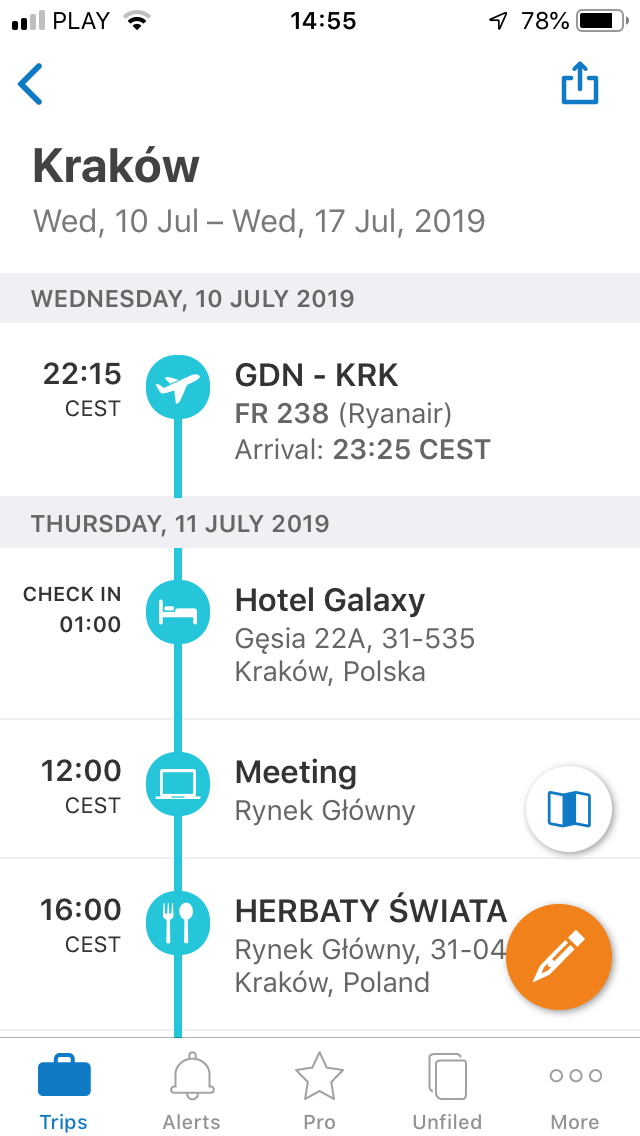
\includegraphics[width=0.4\textwidth]{tripit1}}
\hfill
\subfloat[Opcje transportu taksówką.\label{fig:TIsubim2}]{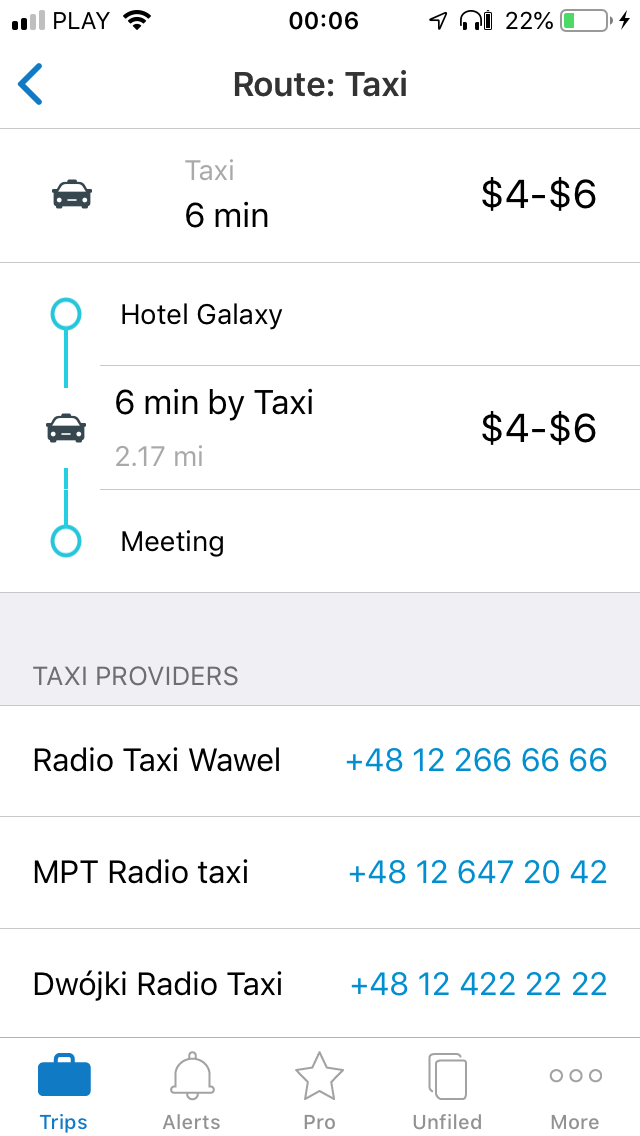
\includegraphics[width=0.4\textwidth]{tripit2}}
\hfill\null

\caption{TripIt: Travel Planner.}
\label{fig:TIimage1}
\end{figure}

\par Oprócz wspomnianego wcześniej automatycznego dodawania rezerwacji i planów przez aplikację po pobraniu tych informacji ze skrzynki pocztowej, można to też było zrobić manualnie. TripIt oferowało 18 różnych elementów, które można było dodać do planu, między innymi: lot (ang. flight), kwatera (ang. lodging), wynajem samochodu (ang. car rental), teatr (ang. theater), rejs (ang. cruise), transport (ang. transportation) i ogólna aktywność (ang. activity). Poszczególne elementy umożliwiały dodanie różnych informacji o planowanej podróży, jednak każdy z nich wymagał dodania daty i godziny do danej aktywności, aby aplikacja mogła je później zorganizować chronologicznie. Przy wpisywaniu niektórych informacji aplikacja podpowiadała jakie słowa mógł mieć na myśli użytkownik, co bywało pomocne. Było tak na przykład w przypadku wpisywania nazwy linii lotniczych i nazwy restauracji, a także w przypadku wybrania pola przeznaczonego na podanie adresu. Była to usługa dostarczana przez firmę Google. Po wybraniu takiego zasugerowanego słowa TripIt często samodzielnie uzupełniał niektóre informacje, takie jak np. adres strony internetowej danego obiektu, czy godzina odprawy samolotowej.
Po dodaniu nowego elementu do planu podróży można go było edytować, usunąć, przenieść do innego planu lub uzupełnić o szczegóły, które nie były dostępne przy tworzeniu np. informacje o rezerwacji (ang. booking info), zdjęcia (ang. photos), uczestnicy (ang. attendees). Dla każdego elementu dostępny był również nawigator (ang. navigator), który po wybraniu miejsca startowego i docelowego wyszukuje możliwe opcje transportu z szacowanym czasem ich trwania i kosztem (w dolarach). Po wybraniu transportu samochodem lub pieszo, aplikacja TripIt przekierowywała do aplikacji Google Maps, gdzie można było zobaczyć wyznaczoną trasę.

\par Ciekawą funkcją było pozyskiwanie informacji o okolicy (ang. neighborhood info), w której znajdował się dodany obiekt. Usługa ta była dostarczana przez GeoSure i udostępniała wskaźniki między innymi z takich kategorii jak: ogólne bezpieczeństwo (ang. overall safety), ryzyko doznania krzywdy fizycznej (ang. physical harm), ryzyko kradzieży (ang. theft). Poza tym TripIt oferowała też wyświetlenie miejsc, będących w pobliżu obiektu z kilku kategorii: restauracje, kawiarnie, bary, bankomaty, parkingi. Wyszukane miejsca pokazywały się na mapie, a po wybraniu jednego z nich można było między innymi zobaczyć godziny otwarcia oraz dodać je do swojego planu podróży.

\begin{figure}[h]

\centering
\null\hfill
\subfloat[Wyszukanie pobliskich kawiarni.\label{fig:TIsubim3}]{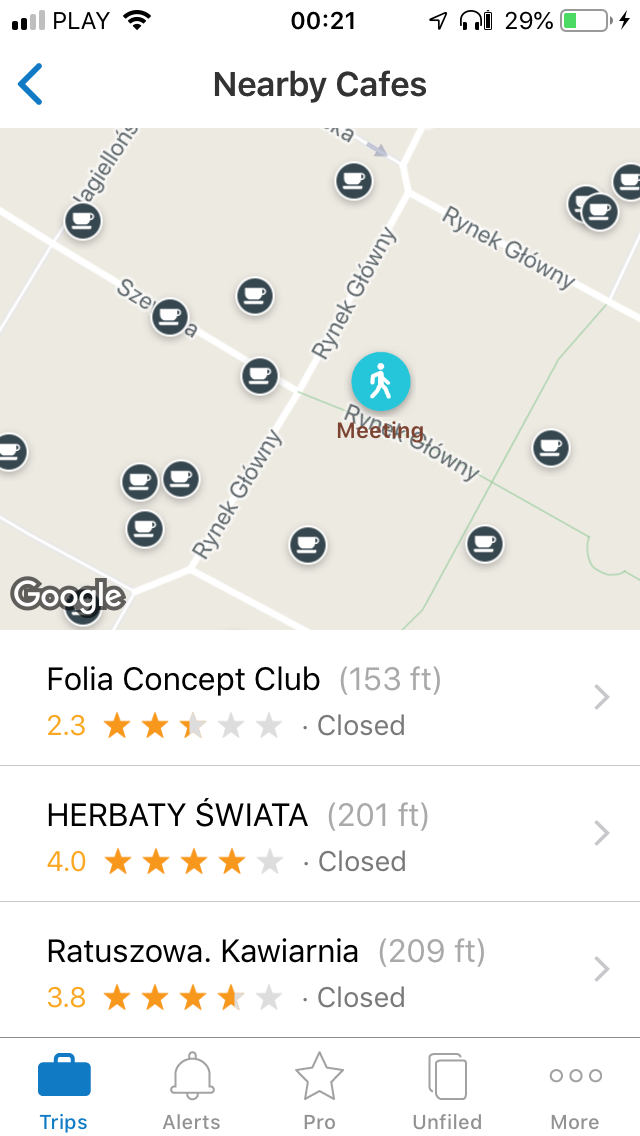
\includegraphics[width=0.4\textwidth]{tripit3}}
\hfill
\subfloat[Udostępnianie planu podróży.\label{fig:TIsubim4}]{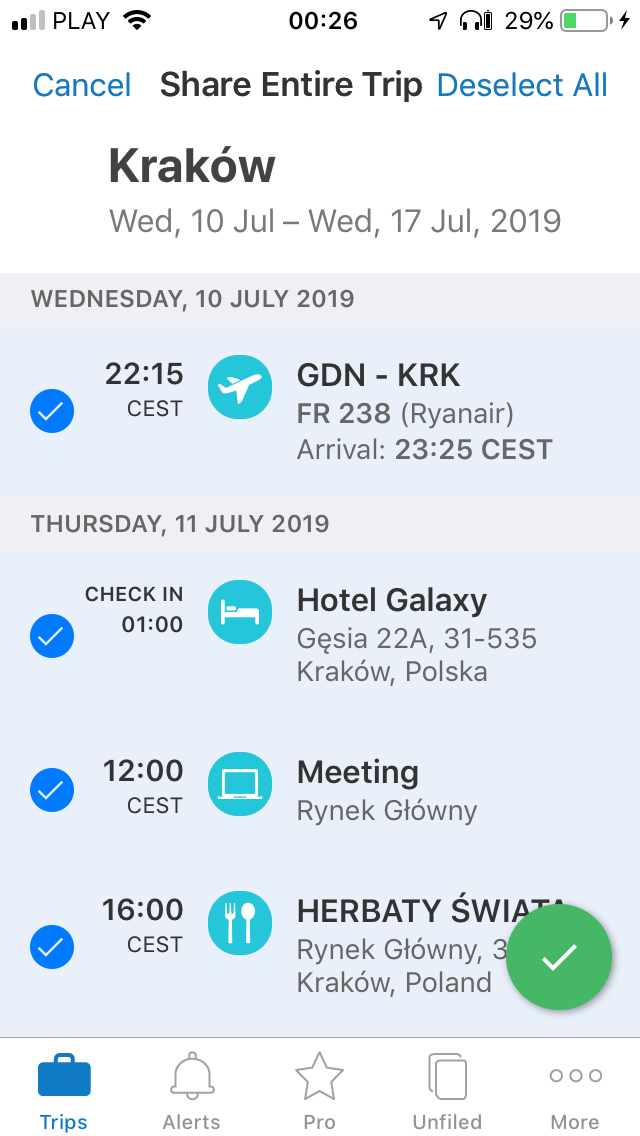
\includegraphics[width=0.4\textwidth]{tripit4}}
\hfill\null

\caption{TripIt: Travel Planner.}
\label{fig:TIimage2}
\end{figure}

\par Każdy plan lub element podróży można było udostępnić lub zapisać w formacie txt. Wybierając opcję Invite Others to View Trip, plan podróży wysyłano na wybrany adres mailowy (który może zostać wyszukany poprzez kontakty) osoby, której można nadać jedno z trzech uprawnień: can view, can edit, can edit and is traveling. W tak wysłanej wiadomości znajdował się link do planu podróży wraz z mapą, które można było wyświetlić w przeglądarce lub aplikacji. W przeglądarce wyświetlała się dodatkowo informacja o pogodzie na każdy dzień podróży. Osoby, którym nadano odpowiednie uprawnienia i posiadały one konto w serwisie TripIt, mogły edytować udostępniony im plan podróży.

\par W aplikacji można było przechowywać informacje o swoich dokumentach i kontaktach, które mogły się przydać w razie nieprzewidzianych sytuacji. Dane te były dostępne po wprowadzeniu 4-cyfrowego pinu, który należało uprzednio ustawić. W ustawieniach można było włączyć synchronizację kalendarza na naszym urządzeniu z aplikacją TripIt, co powodowało automatyczne dodawanie informacji o planie podróży z aplikacji do kalendarza. Dodatkowo w aplikacji można było obejrzeć statystyki ze wszystkich swoich podróży, takie jak liczba przebytych kilometrów, liczba odwiedzonych krajów i inne.

\par Opisane wyżej funkcje dotyczyły darmowej wersji aplikacji TripIt. Wersja Pro rozszerzała tą wersję przede wszystkim o rozbudowany system powiadomień oraz mechanizmów śledzących (ang. trackers). Niektóre z tych udogodnień to: powiadomienia o dostępności lepszych miejsc w samolocie, przypomnienia o konieczności odprawy 24 godziny przed wylotem, wyszukiwanie alternatywnych połączeń, wysyłanie informacji o locie w czasie rzeczywistym podczas całej podróży, udostępnianie interaktywnych map lotniska. Wersję TripIt Pro można było przetestować za darmo przez 30 dni.

\par Aplikacja TripIt oferowała wiele możliwości w planowaniu swoich podróży, co pozwalało na stworzenie bardzo szczegółowych planów. Wiele informacji trzeba było wprowadzać samodzielnie, jednak aplikacja często podpowiadała jakie słowa mógł mieć na myśli użytkownik, co znacznie ułatwiało i przyspieszało ten proces. Dodatkowym ułatwieniem była funkcja automatycznego dodawania danych o rezerwacjach, które mogły być pobierane ze skrzynki pocztowej. Dużą zaletą aplikacji była również opcja wyznaczania trasy między dwoma punktami, jednak koszt takiej wyprawy podawany był tylko w dolarach amerykańskich bez względu na kraj, w którym odbywała się podróż i miejsce zamieszkania użytkownika. TripIt pozwalała w łatwy sposób wyszukać sąsiednie obiekty, takie jak restauracje, czy parkingi, jednak brakowało tu atrakcji turystycznych, a odległość od tych obiektów podawana była w stopach (ft) i nie dało się tego zmienić. Z pewnością przydatną funkcją była możliwość udostępnienia stworzonego przez siebie planu innym osobom, jednak by wysłać link ze sformatowanym planem można było to zrobić jedynie na adres mailowy, a nie przez inne środki komunikacji, gdzie wysłany plan był dostępny wyłącznie w formie tekstowej. Wadą aplikacji była jej dostępność jedynie w języku angielskim. Ponadto cena wersji PRO, która wprowadzała szereg dodatkowych udogodnień, była wysoka i mogła odstraszać potencjalnego użytkownika.

\FloatBarrier
\section{Aplikacja Google Trips -- Travel Planner (Karolina Makuch)}

\par Aplikacja Google Trips – Travel Planner była dostępna na urządzenia mobilne z systemem iOS oraz Android. Była jedną z popularniejszych aplikacji w Sklepie PLAY. Google Trips była także dostępne w Apple Store. 
\par W celu korzystania z Google Trips należało posiadać konto Google. Umożliwiło to dostęp do planu podróży z różnych urządzeń. Niestety aplikacja miała jeden wariant językowy (język angielski).
\par Na samym początku należało wybrać miasto docelowe. Po wyszukaniu miasta, użytkownik miał możliwość nazwania swojej wycieczki oraz dodawania poszczególnych etapów podróży, uwzględniając przedział czasu poświęcony na każdy z nich.

\begin{figure}[h]

\centering
\null\hfill
\subfloat[Tworzenie nowej podróży.\label{fig:GTsubim1}]{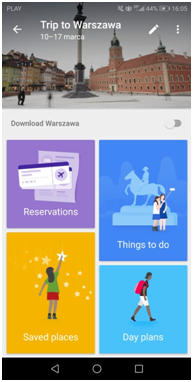
\includegraphics[width=0.4\textwidth]{googletrips1}}
\hfill
\subfloat[Przeglądanie mapy z polecanymi obiektami.\label{fig:GTsubim2}]{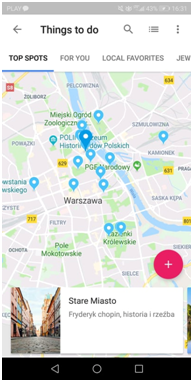
\includegraphics[width=0.4\textwidth]{googletrips2}}
\hfill\null

\caption{Google Trips -- Travel Planner.}
\label{fig:GTimage1}
\end{figure}


\par Aplikacja umożliwiała zapisywanie rezerwacji (ang. Reservations) lotu (ang. Flight), hotelu (ang. Hotel), pociągu (ang. Train), autobusu (ang. Bus), samochodu (ang. Car rental) oraz restauracji (ang. Restaurant). W zależności od rodzaju transportu użytkownik uzupełniał odpowiednie informacje takie jak: skąd chce się wybrać, dokąd, kiedy, o której godzinie, numer telefonu, numer potwierdzający, miejsca pasażerów oraz rodzaj transportu. Google Trips posiadał także Notatnik posiadający ograniczenie do 10 000 słów.
\par Kolejną opcją była możliwość przejrzenia oraz zapisania dostępnych atrakcji (ang. Things to do). Zostały one podzielone na kilka podkategorii na przykład : polecane (ang. Top Spots), preferowane (ang. For you), parki (ang. Parks \& gardens), muzea (ang. Museums), w pomieszczeniu (ang. Indoors), na świeżym powietrzu (ang. outdoor), przyjazne dzieciom (ang. Kids friendly) oraz okoliczne atrakcje (ang. Farther away). Po wybraniu interesującej użytkownika atrakcji użytkownik mógł zobaczyć fotografię, która została wykonana atrakcji, a także miał możliwość przeczytania opisu oraz recenzji użytkowników. Umieszczony był także adres, numer telefonu oraz adres strony internetowej. Aplikacja umożliwiała także nawigację do danej atrakcji. Po naciśnięciu mapy (górny prawy róg) użytkownik mógł zobaczyć lokalizację atrakcji na planie miasta. Daną atrakcję można było zapisać na jednej z domyślnych list: ulubione(ang. favorites), planowane do odwiedzenia (ang. Want to go) oraz ocenione (ang. starred place). Istniała także możliwość stworzenia własnej listy poprzez podanie nazwy.

\par Następny kafelek umożliwiał przejrzenie zapisanych wcześniej atrakcji oraz wyświetlenie ich w wspomnianych wcześniej listach.

\par Aplikacja układała także sugerowane plany dnia (ang. Day plans). Każdy z nich otrzymał własną nazwę. Składał się z mapy, a także ilości oraz odnośników do poszczególnych atrakcji. Aplikacja udzielała użytkownikowi wskazówek odnośnie godzin i dni otwarcia danych atrakcji, ile czasu zazwyczaj spędzają tam zwiedzający, a także jak dużo czasu zajmuje przejście do kolejnego punktu z planu.

\begin{figure}[h]

\centering
\null\hfill
\subfloat[Przeglądanie planu dnia.\label{fig:GTsubim3}]{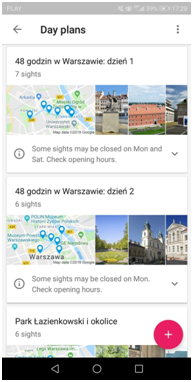
\includegraphics[width=0.4\textwidth]{googletrips3}}\hfill
\subfloat[Przeglądanie informacji na temat regionalnej kuchni.\label{fig:GTsubim4}]{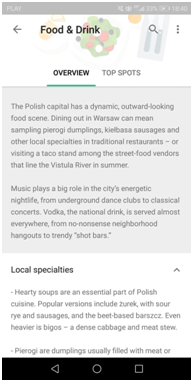
\includegraphics[width=0.4\textwidth]{googletrips4}}\hfill\null

\caption{Google Trips -- Travel Planner.}
\label{fig:GTimage2}
\end{figure}

\par Korzystanie z aplikacji umożliwiało użytkownikom otrzymanie zniżek na poszczególne usługi na przykład: taksówki (ang. pre-booked taxis) czy wypożyczenie samochodu (ang. car hire).
Aplikacja posiadała także informacje na temat lokalnej kuchni (kafelek Food \& Drink). Zawierał on krótki opis charakterystycznej dla danego rejonu kuchni, wypunktowane lokalne specjalności kuchni (ang. local specialities), polecane miejsca do jedzenia „na mieście” (ang. Dining out), a także wskazówki na temat ‘”nocnego życia” (ang. Nightlife). Zakładka „Top Spots” zawierała najbardziej polecane miejsca w poszczególnych kategoriach: ekskluzywne posiłki (ang.high-end dining), budżetowe posiłki (ang. on a budget), miejsca przyjazne rodzinom (ang.family-friendly), śniadania i przekąski (ang. breakfast \& brunch), obiady(ang.lunch),posiłki wegetariańskie (ang.vegetarian-friendly), bary (ang.vodka bars), piwowarnie kraftowe (ang.craft beer) oraz kawiarnie tematyczne (ang.themed cafes). Po wybraniu danej kategorii istniała opcja sortowania propozycji według odległości. Można było także przefiltrować wyniki ze względu na godziny otwarcia (ang. Open now) a także wcześniej zapisanych pozycji (ang. only saved places).
\par Kafelek Zwiedzaj (ang. getting around) umożliwiał sprawdzenie poszczególnych kategorii transportu: on arrival (taxi, ride service, train, bus), public transport (ticket, metro, bus, train, tram), taxi (ang. taxi/ride service), driving, walking \& biking. Każda kategoria była wystarczająco szczegółowo opisana. Zawierała informacje na temat cen, możliwości dojazdu, czasu trwania, możliwych korkach oraz na przykład numerów telefonów do taksówek.
\par Aplikacja zawierała także wskazówki związane z zakupami (ang. Need to know). Informowała użytkownika o najpopularniejszych godzinach otwarcia sklepów, gdzie znajduje się ich najwięcej (ang. Shopping districts). Można było tam także znaleźć przykładowe sklepy (ang. Markets) oraz galerie handlowe (ang. Malls).
 
\begin{figure}[h]

\centering
\null\hfill
\subfloat[Przeglądanie możliwości transportu.\label{fig:GTsubim5}]{
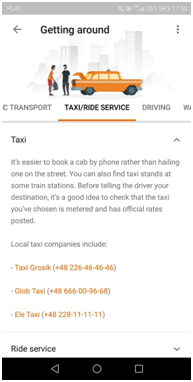
\includegraphics[width=0.4\textwidth]{googletrips5}}
\hfill
\subfloat[Przeglądanie przydatnych informacji.\label{fig:GTsubim6}]{
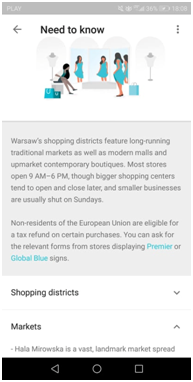
\includegraphics[width=0.4\textwidth]{googletrips6}}
\hfill\null

\caption{Google Trips -- Travel Planner.}
\label{fig:GTimage3}
\end{figure}

\par Zaplanowana przez użytkownika wycieczka została automatycznie przypisana do konta Google. Istniała możliwość udostępnienia jej znajomym. Można było połączyć kilka wycieczek. Po pobraniu informacji na temat danej wycieczki, istniała możliwość powrotu do planu, gdy telefon nie miał dostępu do internetu.
\par Niestety aplikacja była dostępna tylko w języku angielskim. Posiadała także kilka innych wad. Przykładowo podczas wyszukiwania odpowiedniego hotelu aplikacja wyświetla listę miejsc, na której mógł znajdować się sklep meblowy. Brakowało także podpowiedzi przy niektórych polach np. cartype. Aplikacja nie zawsze dodawała informacje z serwisu gmail. Nie można było samemu dodać atrakcji za pomocą informacji z Google Maps, a także dodać ręcznie maili z rezerwacjami.

\FloatBarrier
\section{Sygic Travel -- Planuj podróż (Anna Malizjusz)}

\par Planowanie podróży umożliwia również aplikacja \textit{Sygic Travel: Planuj Podróż}, która została pobrana z serwisu Google Play. Jej duża zaleta to możliwość korzystania z większości funkcji w języku polskim oraz brak konieczności tworzenia konta. Jedyną opcją niedostępną dla niezalogowanego użytkownika była synchronizacja z innymi urządzeniami.
\par Podstawowymi informacjami potrzebnymi do rozpoczęcia planowania podróży były cel, data rozpoczęcia oraz data zakończenia (rys.~\ref{fig:STsubim1}). Opcjonalnie można było podać miejsce przybycia oraz zakwaterowania. Wygodny wybór daty umożliwił wyświetlany kalendarz, a miejsca należało wybrać z podanej listy. Istniała również możliwość filtrowania podanych miejsc po nazwie.
\par Po stworzeniu podróży został wyświetlony interfejs oferujący różne opcje (rys.~\ref{fig:STsubim2}). Po wybraniu mapy można zobaczyć mapę miejsca docelowego z zaznaczonymi atrakcjami. Listę atrakcji można też zobaczyć wybierając opcję miejsca. W obu przypadkach można wybrać kategorie, np. zwiedzanie, zakupy, relaks oraz tagi, np. zwierzęta mile widziane (ang. pets allowed), a także możliwe było dodanie miejsca do odwiedzenia w danym dniu. Dodatkowo zaprezentowano szacunkowy czas dotarcia do celu piechotą z miejsca zakwaterowania. Ta część aplikacji nie została przetłumaczona i była dostępna tylko w języku angielskim. Analogicznie można było przeglądać dostępne kwatery po wybraniu opcji hotele. Dostępne były typowe opcje pomocne w poszukiwaniu zakwaterowania, takie jak wybór średniej oceny, przyznanych gwiazdek, typu zakwaterowania czy udogodnień, np. darmowe Wi-Fi (ang. free hotel Wi-Fi) lub klimatyzacja (ang. air conditioning).

\begin{figure}[h]

\centering
\null\hfill
\subfloat[Tworzenie nowej podróży.\label{fig:STsubim1}]{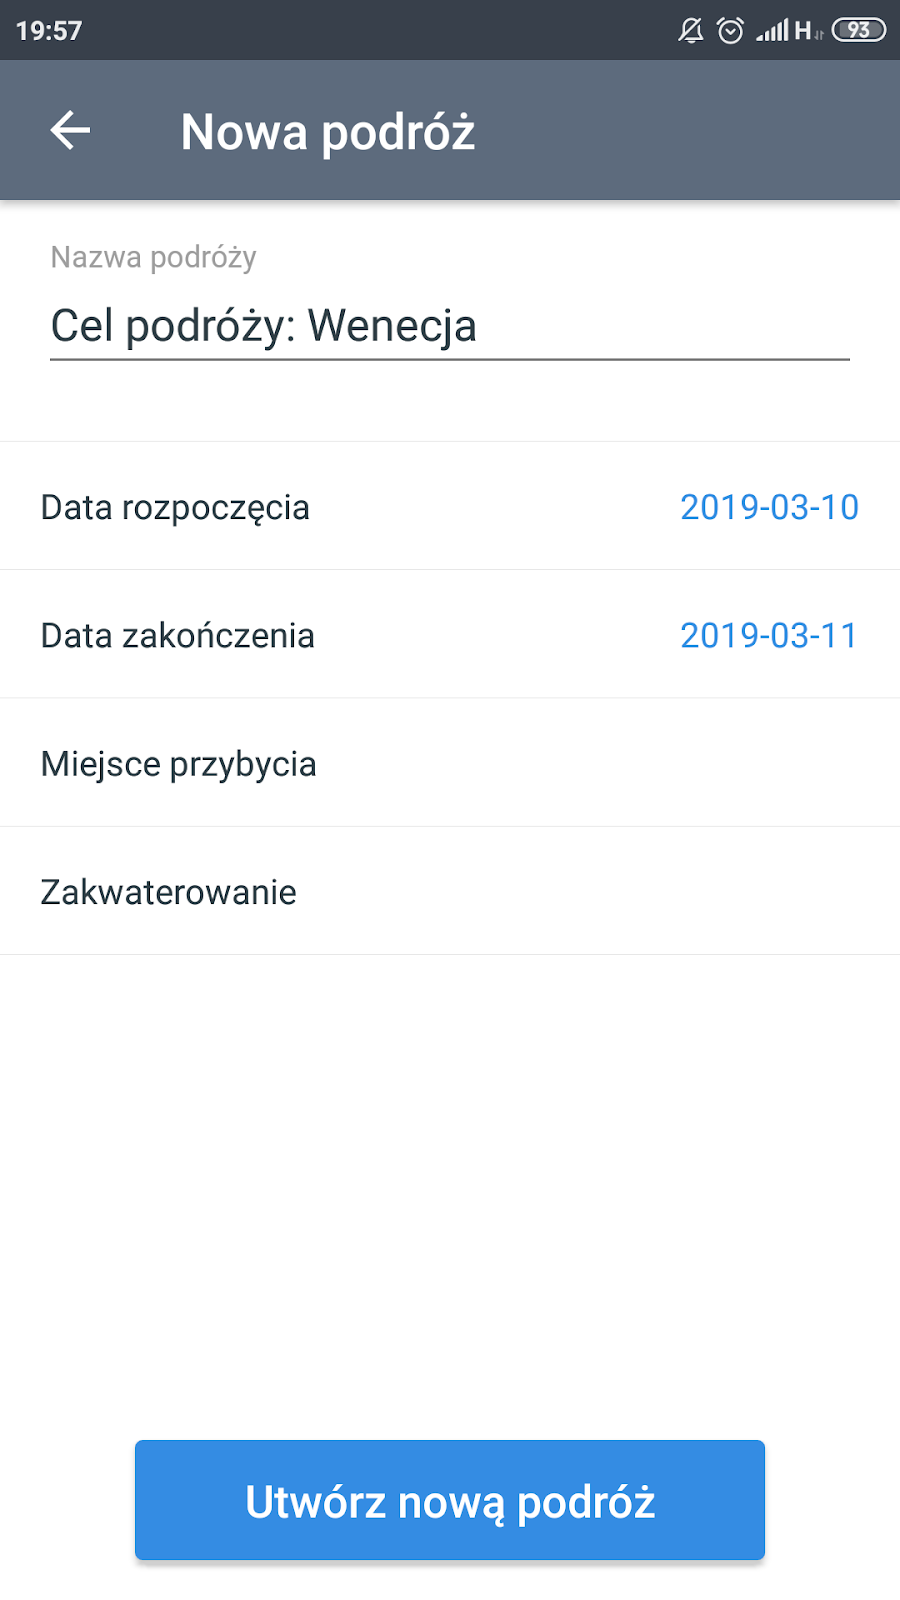
\includegraphics[width=0.4\textwidth]{sygictravel1}}
\hfill
\subfloat[Menu główne.\label{fig:STsubim2}]{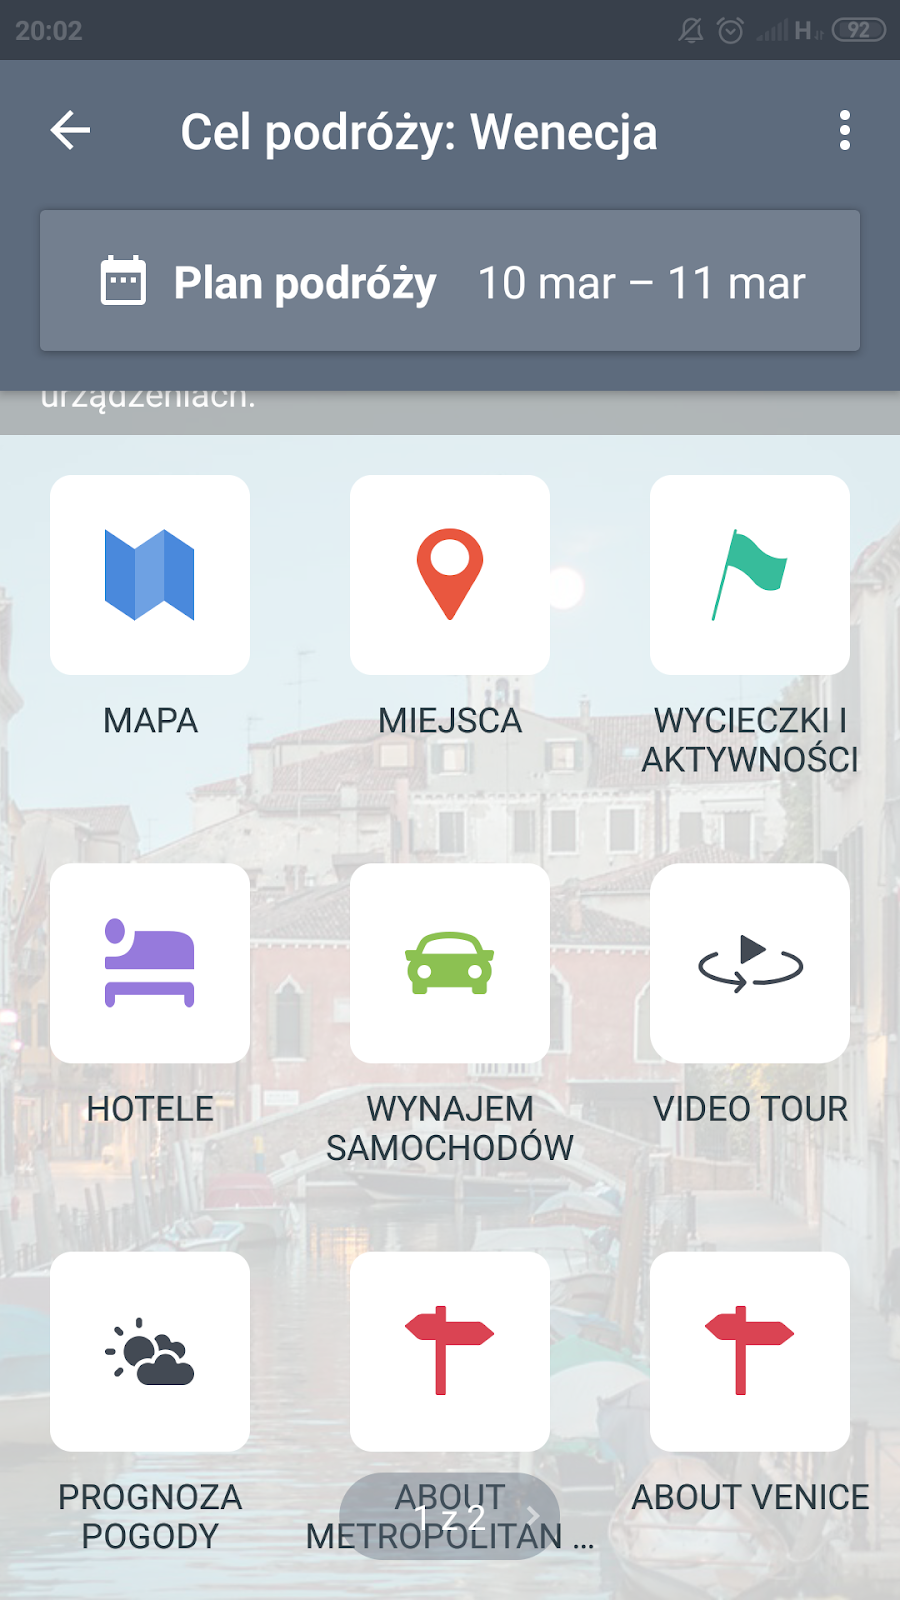
\includegraphics[width=0.4\textwidth]{sygictravel2}}
\hfill\null

\caption{Sygic Travel -- Planuj podróż.}
\label{fig:STimage}
\end{figure}

\par Innego typu funkcjami aplikacji były wycieczki i aktywności oraz wynajem samochodów. Pierwsza opcja umożliwiała wyszukiwanie wycieczek, a także ich rezerwację oraz płatność. Druga wyszukiwała oferty wynajmu samochodów, wyświetlała wszystkie dostępne informacje oraz umożliwiała rezerwację. W obu funkcjach udostępniono możliwość filtrowania wyników. Poważną wadą wyszukiwarki samochodów do wynajęcia stanowił niejasny komunikat o błędzie w przypadku podania dat z przeszłości, który sugerował sprawdzenie zaznaczonych pól nie wskazując możliwego rozwiązania problemu.
\par Kolejna ciekawa opcja to wycieczka wideo (ang. video tour), która była dostępna tylko dla bardziej popularnych celów podróży. Po wybraniu tej opcji użytkownikowi wyświetlany był film wraz z angielskim komentarzem z jednodniowej wycieczki po wybranym mieście. Prezentowano charakterystyczne i warte odwiedzenia zabytki i atrakcje turystyczne, a użytkownikowi umożliwiono ingerowanie w pokazywany obraz. Filmy oferowały widok 360° po obróceniu telefonu.
\par Trzy kolejne funkcje były czysto informacyjne, lecz przydatne. Pokazywały prognozę pogody na najbliższe 14 dni, a także informacje o mieście i okolicy. Obszerność tych danych różniła się w zależności od popularności celu podróży, ale mogła stanowić dobrą podstawę dla nieobeznanych z miejscem użytkowników. Informacje w języku angielskim zostały zaczerpnięte z serwisu Wikivoyage, który można otworzyć w aplikacji oraz przeglądarce internetowej.
\par Po zakupie \textit{Sygic Travel Premium} za 88,99 zł pojawiały się dodatkowe funkcjonalności, takie jak zapisanie mapy miejsca docelowego do użytku offline. Kolejną opcją było wyświetlenie informacji o zabytkach, hotelach i atrakcjach, których odwiedzenie proponowała aplikacja. Darmowa wersja oferowała wszystkie najbardziej potrzebne opcje, więc zakup rozszerzonej wersji nie był koniecznością, a jedynie nieznacznym zwiększeniem możliwości aplikacji.
\par Aplikacja została zintegrowana z innymi produktami firmy Sygic. Przy każdym miejscu oferowała możliwość nawigacji przy pomocy Sygic GPS Navigation \& Maps, a rezerwacja wycieczek i samochodów była wspierana przez witrynę \textit{Sygic Travel}, która była dostępna również z komputera z przeglądarki internetowej.
\par \textit{Sygic Travel} to spełniające podstawowe funkcje narzędzie ułatwiające planowanie podróży. Nie oferowała wielu możliwości, jednak warto zauważyć, że większość z nich była dostępna w wersji podstawowej i nie zmuszała użytkownika do zakupu stosunkowo drogiej wersji premium. Udostępniała bogaty wybór możliwych do odwiedzenia miejsc w wybranym celu podróży, a sam cel mógł należeć do egzotycznych, np. Udaipur w Indiach. Podstawowe informacje, takie jak mapa, atrakcje turystyczne czy prognoza pogody były zawsze dostępne. 

\FloatBarrier
\section{Expedia (Magdalena Solecka)}
\par Kolejna aplikacja do planowania podróży to \textit{Expedia}, dostępna na urządzeniach z systemem iOS oraz Android. Korzystanie z niej było możliwe po założeniu konta użytkownika. Wśród dostępnych tłumaczeń nie znajdował się język polski. Aplikacja składała się z czterech głównych funkcjonalności \ref{fig:Esubim1} rezerwacja noclegu (ang. Hotels), rezerwacja lotu (ang. Flights), rezerwacja samochodu (ang. Cars) oraz wyszukiwanie ciekawych miejsc w okolicy (ang. Thing to Do). Nie było możliwości wyszukania restauracji w rejonie ani transportu naziemnego, koleją lub autobusem.

\begin{figure}[h]

\centering
\null\hfill
\subfloat[Menu główne.\label{fig:Esubim1}]{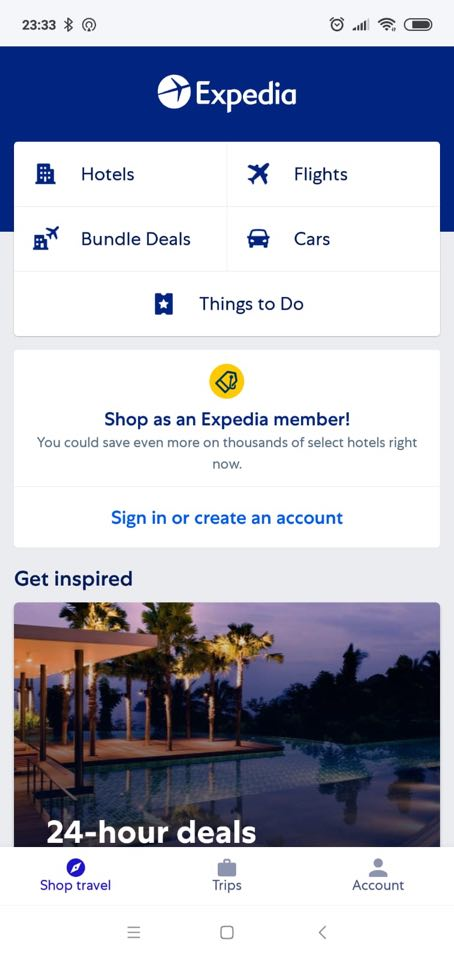
\includegraphics[width=0.4\textwidth]{expedia1}}
\hfill
\subfloat[Wyszukiwanie noclegu.\label{fig:Esubim2}]{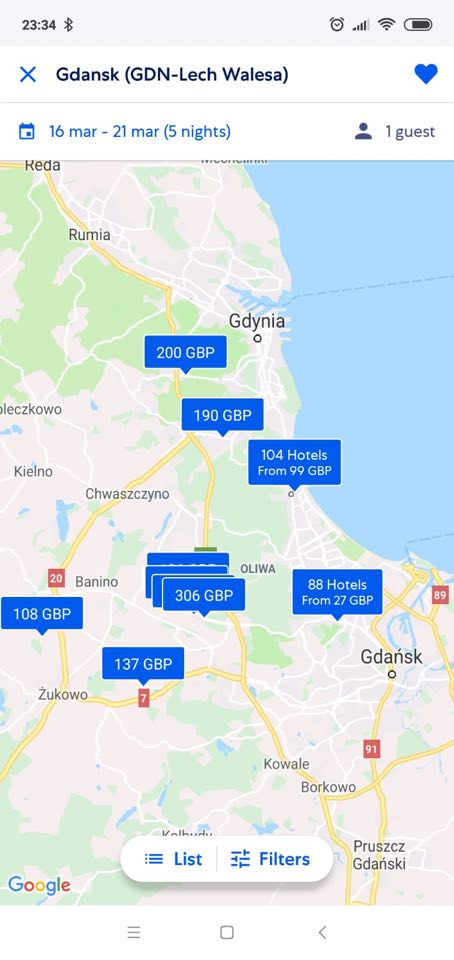
\includegraphics[width=0.4\textwidth]{expedia2}}
\hfill\null

\caption{Expedia.}
\label{fig:Eimage}
\end{figure}

\par W celu wyszukania noclegu należało podać następujące dane: datę zameldowania i wymeldowania, miasto docelowe podróży, liczbę pokoi oraz osób do zakwaterowania. Zaprezentowane przez aplikację wyniki mogły zostać posortowane po cenie lub recenzjach użytkowników, a także przefiltrowane względem darmowego anulowania rezerwacji, śniadaniu wliczonym w cenę pobytu, klimatyzacją czy Wi-Fi. Wygodnym rozwiązaniem była mapka \ref{fig:Esubim2} z naniesionymi na nią punktami z ceną w miejscu, w którym znajdował się oferowany pokój, co umożliwiało łatwiejszą ocenę odległości od centrum.
\par W przypadku rezerwacji miejsca w samolocie można było wyszukać lot w jedną lub obie strony. Należało podać miejsce wylotu i przylotu oraz daty. Przedstawione wyniki można było porządkować według rosnącego kosztu. Aplikacja nie dawała możliwości porównania cen w różnych dniach np. w formie kalendarza uzupełnionego najniższymi cenami w danym dniu, co przy podróżowaniu z niskim budżetem byłoby pomocne. Możliwe było równoczesne wyszukanie lotów oraz noclegu (ang. Bundle Deals).
\par Aplikacja oferowała również możliwość wypożyczenia samochodu. Tak jak w poprzednich dwóch przypadkach należało podać przedział czasu korzystania z pojazdu, miejsce odbioru i pozostawienia. Wyświetlone informacje o pojazdach były przydatne przy dokonywaniu wyboru, automatyczna czy manualna skrzynia biegów, ilość pasażerów.Dostępne sortowanie po cenie.
\par Ostatnia funkcjonalność, wyszukiwanie atrakcji, zabytków, ciekawych wydarzeń. Wymagane ramy czasowe oraz lokalizacja. Rezultaty mogły być przeglądane po cenie lub popularności. Nie umożliwiono użytkownikowi oceny odległości między zaproponowanymi miejscami tak jak w przypadku noclegu, ale pomocny był przybliżony czas, który należy przeznaczyć na każdą z atrakcji.
\par Wszystkie rezerwacje wykonane za pomocą aplikacji \textit{Expedia}, można było przeglądać w zakładce Wycieczki (ang. Trips) i takim zestawem dzielić się ze współtowarzyszami podróży również korzystających z aplikacji.
